\subsection{Формула Эйлера}
\begin{theorem}
    Для любого выпуклого многогранника выполнено \[B - P + \Gamma = 2.\]
\end{theorem}
\begin{proof}
    Сведём доказательство формулы Эйлера для выпуклых многогранников к доказательству формулы Эйлера для плоских графов.

    Нужно так спроектировать многогранник, чтобы граф, получившийся в результате проекции, был плоским. Эту идею можно довести до аккуратного доказательства, если рассматривать строго выпуклый многогранник, но мы будем делать иначе.

    Рассмотрим две проекции. Пусть $L$ — многогранная поверхность, задающая многогранник $M$.

    1) $\pi: L \to S^2$.

    Спроектируем поверхность многогранника из некоторой внутренней точки многогранника $O$ на сферу с центром в этой точке (выберем сферу достаточно большого радиуса, чтобы многогранник в ней полностью содержался).

    \begin{figure}[h]
        \centering
        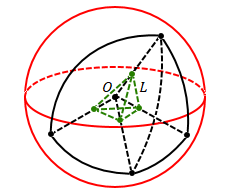
\includegraphics[scale=0.8]{images/c7.2.png}
        \caption{Проекция многогранника на сферу.}
        \label{fig:c7.2}
    \end{figure}

    Докажем, что отображение $\pi$ будет взаимно-однозначным (для этого нужно понять, что луч с началом в точке $O$ ровно один раз пересечёт поверхность многогранника).

    Докажем, что луч с началом в точке $O$ пересечёт поверхность многогранника. Так как $O$ — внутренняя точка многогранника, то существует шар с центром в точке $O$ (окрестность точки $O$), целиком лежащий в многограннике, поэтому начало и некоторая окрестность луча принадлежат многограннику. Также на этом луче будут точки, не принадлежащие многограннику, поэтому существует точка на границе многогранника, принадлежащая лучу (супремум множества точек, принадлежащих многограннику).

    Докажем, что луч пересечёт ровно один раз: допустим, луч пересекает поверхность многогранника в двух точках $A$ и $B$. Как отмечалось выше, существует шар с центром в точке $O$, целиком лежащий внутри многогранника. Рассмотрим конус над этим шаром с вершиной в точке $B$. Очевидно, что $A$ — внутренняя точка этого конуса, т.е. существует шар с центром в точке $A$, целиком лежащий внутри этого конуса (если $A$ лежит вне конуса, то рассмотрим конус с вершиной в точке $A$ —  в этом случае $B$ будет внутренней точкой конуса).

    \begin{figure}[h]
        \centering
        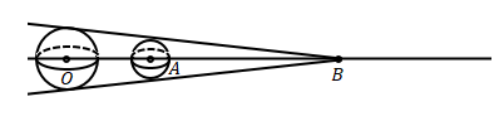
\includegraphics[scale=0.8]{images/c7.3.png}
        \caption{$A$ — внутренняя точка конуса.}
        \label{fig:c7.3}
    \end{figure}

    Так как многогранник выпуклый, то весь конус принадлежит многограннику, поэтому шар с центром в точке $A$ — это окрестность точки $A$, целиком состоящая из точек, принадлежащих многограннику, откуда следует. что $A$ — внутренняя точка многогранника — противоречие.

    Итак, в результате проекции $\pi: L \to S^2$ получаем граф на сфере — каждой вершине многогранника будет соответствовать точка на сфере, каждому ребру многогранника — дуга окружности, являющаяся пересечением плоскости, проходящей через точку $O$, со сферой.

    2) $p: S^2 \setminus C \to \R^2$.

    \begin{figure}[h]
        \centering
        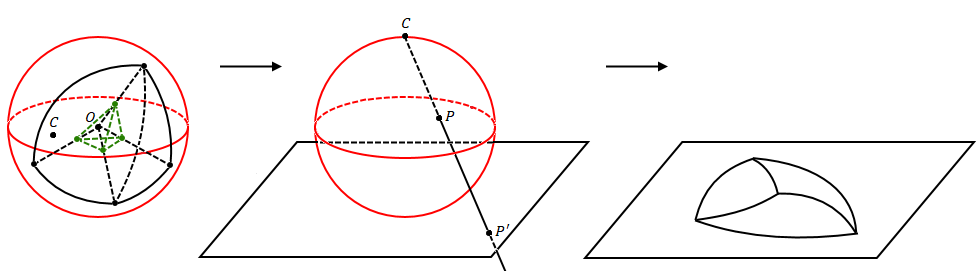
\includegraphics[scale=0.5]{images/c7.4.png}
        \caption{Стереографическая проекция.}
        \label{fig:c7.4}
    \end{figure}

    Теперь рассмотрим проекцию сферы на плоскость. Выберем точку $C$ на сфере, не принадлежащую ни одному из рёбер, и рассмотрим стереографическую проекцию из этой точки — получим некоторый плоский граф, причём каждой вершине графа на сфере будет соответствовать вершина графа на плоскости, каждому ребру — ребро, каждой области на сфере, на которые граф разбивал сферу, будет соответствовать область на плоскости, причём области, содержащей точку $C$, будет соответствовать неограниченная область на плоскости.

    Итак, мы получили взаимно-однозначное соответствие между вершинами и рёбрами исходного многогранника и вершинами и рёбрами полученного графа, поэтому формула Эйлера для плоских графов верна и для выпуклых многогранников.

    Как делать не надо: если мы спроектируем многогранник на плоскость, то получим некоторый граф. При проекции вершины многогранника перейдут в вершины графа, рёбра — в рёбра, каждой грани многогранника будет соответствовать компонента связности на плоскости, поэтому формула Эйлера для многогранника будет верна, поскольку она верна для плоского графа.

    \begin{figure}[h]
        \centering
        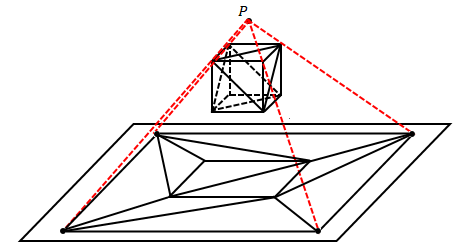
\includegraphics[scale=0.8]{images/c7.1.png}
        \caption{Проекция куба с фиктивными рёбрами.}
        \label{fig:c7.1}
    \end{figure}

    Это рассуждение проходит не для всех выпуклых многогранников — например, если подразбить все грани куба на треугольники, как показано на рис.\ref{fig:c7.1}, то граф, полученный в результате проекции, не будет вложенным.
\end{proof}

\subsection{Правильные многогранники}
\begin{definition}
    Правильный многогранник — это выпуклый многогранник, грани которого — это равные правильные многоугольники, все двугранные углы которого равны.
\end{definition}

\begin{remark}
    Все двугранные углы равны $\Longleftrightarrow$ в любой вершине сходится одинаковое число рёбер.
\end{remark}

Почему можно заменить? Потому что верна следующая теорема:

\begin{theorem}[Коши]
    Два выпуклых многогранника с одинаковым комбинаторным строением, имеющие равные соответствующие грани, совмещаются движением пространства (т.е. конгруэнтны).
\end{theorem}
\begin{proof}
    Без доказательства.
\end{proof}

\begin{theorem}
    В пространстве существует ровно пять правильных многогранников (платоновы тела): тетраэдр, куб, октаэдр, икосаэдр, додекаэдр.
\end{theorem}
\begin{proof}
    Будем рассматривать множество вершин и рёбер многогранника как некоторый граф, для которого верно соотношение \[B - P + \Gamma = 2.\]

    Теперь используем условие правильности многогранника. Пусть $n$ — количество сторон в каждой грани, $k$ — количество рёбер, сходящихся в вершине. Тогда можно двумя способами подсчитать количество рёбер. Действительно, в каждую вершину входит $k$ рёбер, тогда $B \cdot k$ — удвоенное количество рёбер (каждое ребро посчитали дважды), поэтому \[2P = B \cdot k.\]
    
    С другой стороны, у каждой грани $n$ рёбер, тогда $\Gamma \cdot n$ — удвоенное количество рёбер (каждое ребро принадлежит ровно двум граням), поэтому \[2P = \Gamma \cdot n.\]

    Выражая из полученных соотношений число вершин $B$ и число граней $\Gamma$ и подставляя в формулу Эйлера, получим:
    \[\frac{2P}{k} - P + \frac{2P}{n} = 2 \Longleftrightarrow \frac{2}{k} + \frac{2}{n} = 1 + \frac{2}{P}.\]

    Так как $P,n,k$ — целые числа, а из геометрических соображений понятно, что $n \geq 3, \ k \geq 3$, то левая часть равенства при больших $k, \ n$ меньше 1, а правая часть больше 1. (Нет, ну это уже) перебор:

    \[n = 3 \Longrightarrow \frac{2}{k} = \frac{1}{3} + \frac{2}{P} \Longrightarrow k \leq 5 \Longrightarrow k = 3,4,5\]
    \[n = 4 \Longrightarrow \frac{2}{k} = \frac{1}{2} + \frac{2}{P} \Longrightarrow k \leq 3 \Longrightarrow k = 3\]
    \[n = 5 \Longrightarrow \frac{2}{k} = \frac{3}{5} + \frac{2}{P} \Longrightarrow k \leq 3 \Longrightarrow k = 3\]
    \[n \geq 6 \Longrightarrow \frac{2}{k} = \frac{2}{3} + \frac{2}{P} \Longrightarrow k \leq 2 \Longrightarrow \text{решений нет}.\]

    Всего получили 5 вариантов: тетраэдр ($n = 3, \ k = 3$), октаэдр ($n = 3, \ k = 4$), икосаэдр ($n = 3, \ k = 5$), куб ($n = 4, \ k = 3$), додекаэдр ($n = 5, \ k = 3$).

    \begin{figure}[h]
        \centering
        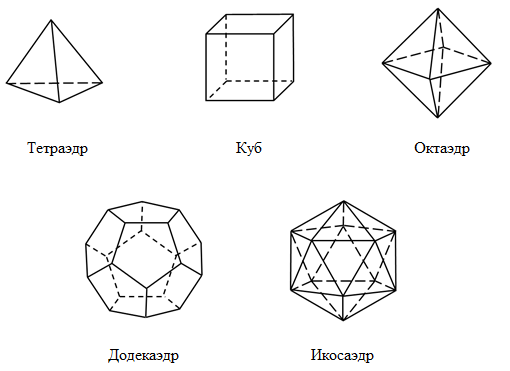
\includegraphics[scale=0.8]{images/c7.5.png}
        \caption{Правильные многогранники.}
        \label{fig:c7.5}
    \end{figure}



    % Все грани — правильные $n$-угольники и в любой вершине сходятся $m$ рёбер.

    % \[\begin{cases}
    %     n \gamma = 2 P, \\
    %     m B = 2 P, \\
    %     B - P + \Gamma = 2.
    % \end{cases} \Longrightarrow\]
    
    % $$\frac{2 P}{m} - P + \frac{2 P}{n} = 2 \Longrightarrow P \left(\frac{2}{m} + \frac{2}{n} - 1 \right) = 2$$
    % $$\frac{2}{m} + \frac{2}{n} > 1$$
    % при $m > 6$: $\frac{2}{m} \leq \frac{1}{3}$ и $\frac{2}{n} > \frac{2}{3} \Longrightarrow n < 3$ — противоречие, т.к. если $n \geq 6 \Longrightarrow m < 3$ — не бывает.
\end{proof}

% Классификация многогранников:
% \begin{enumerate}
%     \item $n = 3, \ m = 3$: $P \left(\frac{2}{3} + \frac{2}{3} - 1 \right) = 2 \Longrightarrow P = 6 \Longrightarrow \Gamma = \frac{2  \cdot 6}{3} = 4$
% \end{enumerate}

\subsection{Теоремы Сабитова и Минковского}
\begin{definition}
    \textit{Деформация многогранника} — это непрерывное отображение из одного многогранника в другой, которое сохраняет сохраняет комбинаторную структуру многогранника.
\end{definition} 
\begin{definition}
    \textit{Изгибание многогранника} — это непрерывная деформация, которая сохраняет длины всех рёбер многогранника.
\end{definition} 
\begin{example}
    Деформация куба в прямоугольный параллелепипед — деформация, но не изгибание. Гомотетия многогранника — изгибание.
\end{example}
\begin{theorem}[Сабитов]
    При изгибании невыпуклого многогранника его объём сохраняется.
\end{theorem}
\begin{proof}
    Временно идея доказательства: Формула Герона:
    \[S^2 = p(p - a)(p - b)(p - c).\]
    Если рассматривать правую часть данной формулы как многочлен, коэффициенты которого зависят от длин сторон, то корень этого многочлена является квадратом площади треугольника.

    Аналогичная формула существует и для тетраэдра: если задать длины всех сторон тетраэдра, то можно предъявить многочлен, коэффициенты которого зависят только от длин сторон, а корнем этого многочлена является объём тетраэдра.

    Оказывается, для любого многогранника существует многочлен, коэффициенты которого зависят только от длин сторон многогранника, корнем которого является объём многогранника. Отсюда следует, что при изгибании многогранника его объём будет сохраняться, так как длины всех рёбер сохраняются при изгибании.
\end{proof}

Рассмотрим произвольный многогранник. Пусть $S_i$ — площадь его $i$-й грани, $\overrightarrow{n_i}$, $|\overrightarrow{n_i}| = 1$ — внешняя единичная нормаль к $i$-й грани.

\begin{statement}
    Для любого строго выпуклого многогранника набор $\overrightarrow{n_1}, \dots, \overrightarrow{n_k}$, $\ S_1, \dots, S_k$, где $\overrightarrow{n_i}$ — единичные нормали, а $S_i$ — площади граней, удовлетворяет следующим условиям:
    \begin{enumerate}
        \item $\overrightarrow{n_1}, \dots, \overrightarrow{n_k}$ не лежат в одном замкнутом полупространстве;
        \item \[\sum_{i=1}^{k}S_i \overrightarrow{n_i} = 0.\]
    \end{enumerate}
    Набор, который удовлетворяет данным условиям, называется \textit{ежом}.

    \begin{figure}[ht]
        \centering
        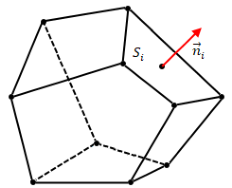
\includegraphics[scale=0.8]{images/c7.6.png}
        \caption{Ёж.}
        \label{fig:c7.6}
    \end{figure}
\end{statement}
\begin{proof}
    Докажем сначала второе утверждение. Рассмотрим некоторую внутреннюю точку многогранника $O$, и в каждой грани выберем внутреннюю точку грани $P_i$. Разобьём многогранник на пирамиды с вершиной в точке $O$, основаниями которых являются грани многогранника. Если многогранник выпуклый, то эти пирамиды не пересекаются, а их объединение дает весь многогранник.

    Объем пирамиды с вершиной $O$, основанием которой является $i$-ая грань, равен
    $$V_{\Pi}=\frac{1}{3} S_i\left(\overrightarrow{O P_i}, \overrightarrow{n_i}\right)$$

    Действительно, $\left(\overrightarrow{O P_i}, \overrightarrow{n_i}\right)$ — это длина проекции отрезка $\overrightarrow{O P_i}$ на нормаль к грани, то есть, высота пирамиды. Тогда объем многогранника равен
    $$V=\sum_{i=1}^k \frac{1}{3} S_i\left(\overrightarrow{O P_i}, \overrightarrow{n_i}\right)=\frac{1}{3} \sum_{i=1}^k\left(\overrightarrow{O P_i}, S_i \overrightarrow{n_i}\right)$$

    Для другой точки $O^{\prime}$ мы получим аналогичную формулу:
    $$V=\sum_{i=1}^k \frac{1}{3} S_i\left(\overrightarrow{O^{\prime} P_i}, \overrightarrow{n_i}\right)=\frac{1}{3} \sum_{i=1}^k\left(\overrightarrow{O^{\prime} P_i}, S_i \overrightarrow{n_i}\right)$$
    Значит,
    $$\sum_{i=1}^k\left(\overrightarrow{O P_i}, S_i \overrightarrow{n_i}\right)=\sum_{i=1}^k\left(\overrightarrow{O^{\prime} P_i}, S_i \overrightarrow{n_i}\right)$$
    откуда
    $$\sum_{i=1}^k\left(\overrightarrow{O P_i}-\overrightarrow{O^{\prime} P_i}, S_i \overrightarrow{n_i}\right)=0 \Longleftrightarrow \sum_{i=1}^k\left(\overrightarrow{O O^{\prime}}, S_i \overrightarrow{n_i}\right)=0$$

    Вынося вектор $\overrightarrow{O O^{\prime}}$ за скобки, получаем
    $$\left(\overrightarrow{O O^{\prime}}, \sum_{i=1}^k S_i \overrightarrow{n_i}\right)=0$$

    Так как это верно для любых внутренних точек многогранника $O$ и $O^{\prime}$, то
    $$\sum_{i=1}^{k} S_i \overrightarrow{n_i} = 0.$$

    Теперь докажем первое утверждение. Допустим, векторы $S_i \overrightarrow{n_i}$ лежат в одном замкнутом полупространстве. Тогда, поскольку их сумма равна нулю, они должны лежать в одной плоскости: действительно, так как они лежат в замкнутом полупространстве, то их проекции на ось $x$ будут неотрицательными. С другой стороны, их сумма равна нулю, поэтому их проекции на ось $x$ равны нулю, то есть, они лежат в одной плоскости. Иными словами, все они перпендикулярны некоторой прямой.

    \begin{figure}[ht]
        \centering
        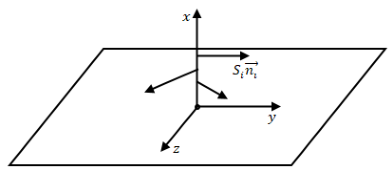
\includegraphics[scale=0.8]{images/c7.7.png}
        \caption{Вектора $S_i \overrightarrow{n_i}$ лежат в одной плоскости.}
        \label{fig:c7.7}
    \end{figure}

    Но это невозможно, потому что это означает, что все грани параллельны некоторой прямой, откуда следует, что все рёбра перпендикулярны некоторой прямой, тогда в любой вершине могут сходиться максимум два ребра.
\end{proof} 

Мы доказали, что по многограннику можно построить некоторого ежа. Оказывается, обратное утверждение тоже верно:

\begin{theorem}[Минковский]
    Пусть дан набор векторов $\overrightarrow{n_1}, \dots, \overrightarrow{n_k}$, никакие два из которых не сонаправлены и не лежат в одном полупространстве, и набор чисел $S_1, \dots, S_k$, что $\sum S_i \overrightarrow{n_i} = 0$. Тогда существует ровно один строго выпуклый многогранник, для которого векторы $S_i \overrightarrow{n_i}$ являются его ежом.
    % (вот тут дополни про фиктивные вершины "фиктивная вершина — вершина, в которой сумма плоских углов равна два пи")
\end{theorem}
\begin{proof}
    Без доказательства.
\end{proof}